\documentclass[11pt,a4paper]{article}

\usepackage{amsmath,amssymb,amsfonts}
\usepackage{graphicx}
\usepackage{booktabs}
\usepackage{hyperref}
\usepackage[margin=2.5cm]{geometry}
\usepackage{parskip}
\usepackage{setspace}

\onehalfspacing

\title{How Far Does the Model Hold?\\
Robustness of Multihorizon Battery Failure Intelligence\\
Under Realistic Operating Conditions}

\author{Tareq Anwar Shikdar\textsuperscript{*}\thanks{Corresponding author.} \and Hannu Laaksonen\\
Flexible Energy Resources / Electrical Engineering,\\
School of Technology and Innovations, University of Vaasa, Finland\\
\{tareq.shikdar, hannu.laaksonen\}@uwasa.fi}

\begin{document}

\maketitle

\begin{abstract}
Multihorizon hazard learning produces calibrated failure probabilities that enable risk-aware battery dispatch, but existing validation uses only clean laboratory cycling data. We test whether calibration survives under realistic operating conditions. Using the published XGBoost hazard model trained on NASA 18650 data, we generate synthetic perturbed profiles at four severity levels by truncating raw discharge curves to simulate partial cycling (DoD 15--100\%), adding temperature noise ($\sigma=0.5$--$3.0^\circ$C), and randomizing rest effects. The fixed model's calibration degrades substantially across all four horizons (10, 20, 30, 50 cycles): ECE rises from 0.01--0.03 to 0.27--0.38, while AUC drops from 0.99--1.00 to 0.61--0.77. Degradation saturates at the mildest perturbation---even minimal partial cycling causes near-maximal calibration loss. Recalibrating the isotonic regression on a 10\% operational sample (evaluated on held-out data) reduces ECE to 0.06--0.09, recovering 71--88\% of the calibration gap. Calibration is not inherently robust to observational shifts, but a minimal recalibration step suffices for field deployment.
\end{abstract}

\section{Introduction}

Battery energy storage systems (BESSs) are dispatched for flexibility services in renewable-dominated power systems. Operators need to know not just how much energy a battery can deliver, but whether it can reliably complete a scheduled service. The multihorizon hazard learning framework~\cite{shikdar2026learning} addresses this by estimating the probability of failure within predefined service horizons (10, 20, 30, 50 cycles). With isotonic regression calibration, it achieved a 71\% reduction in operational failures (from 10.3\% to 2.95\%) in cross-validated lab experiments.

But the model was trained exclusively on clean laboratory data---full cycles at fixed C-rates, consistent rest periods, controlled temperatures. Real BESS operation involves partial cycles at varying depths of discharge (DoD), irregular loads, random rest periods, and temperature fluctuations. The calibration quality under these conditions is unknown, and no operator can trust a model whose reliability degrades in uncharacterized ways.

\textbf{Practical takeaway for operators.} Deploying a lab-trained hazard model directly into field operation risks systematically overconfident failure probabilities---the calibration error jumps from near-zero to 0.27--0.38 under partial cycling (Section~\ref{sec:results}). However, the fix does not require retraining the base model. An operator need only collect 50--100 operational cycles, extract the same per-cycle features, run the frozen model, and fit a new calibrator (isotonic or Platt) on the resulting raw probabilities. This recalibration step recovers 71--88\% of the calibration gap (ECE drops to 0.06--0.09), and isotonic and Platt perform equivalently across all horizons (Section~\ref{sec:recal}). Temperature scaling---a single-parameter logistic adjustment---is only competitive at the shortest horizons (H $\leq$ 20); isotonic or Platt is recommended for longer prediction windows.

This paper tests whether calibration survives realistic conditions. We generate perturbed operational data from existing lab cycling data, measure calibration degradation across four severity levels and four prediction horizons, and test whether lightweight recalibration can restore trustworthiness. The true SOH trajectory is preserved throughout, isolating the effect of observational distribution shift from changed degradation dynamics.

\section{Background}

The framework~\cite{shikdar2026learning} defines operational failure as the inability to complete a service commitment within horizon \(H\) cycles. A gradient-boosted tree ensemble (XGBoost) maps per-cycle features to failure probability:

\[
f_\theta: \mathbf{x}_t \longrightarrow P_{\text{fail}}(t, H)
\]

where \(\mathbf{x}_t = \{\text{SOH}_t, V_{\text{avg}}, V_{\text{min}}, I_{\text{avg}}, T_{\text{avg}}, \text{duration}, t\}\). After training, isotonic regression calibrates raw probabilities. Model parameters are in Table~\ref{tab:params} and match the original framework~\cite{shikdar2026learning}.

\begin{table}[htbp]
\centering
\caption{Model parameters.}
\label{tab:params}
\begin{tabular}{@{}ll@{}}
\toprule
Parameter & Value \\
\midrule
Model type & XGBoost \\
Estimators & 300, max depth 4, lr 0.05 \\
Subsample / colsample & 0.8 / 0.8 \\
Min child weight & 5 \\
Calibration & Isotonic regression \\
\bottomrule
\end{tabular}
\end{table}

Calibration matters because dispatch decisions use risk thresholds. A well-calibrated model satisfies \(P(\text{failure} \mid \hat{P}=p) \approx p\); without this, systematic biases cause unsafe decisions regardless of AUC. ECE quantifies this mismatch across 10 uniform bins. Figure~\ref{fig:reliability} illustrates the calibration degradation conceptually as distribution shift moves predictions off the diagonal.

\subsection{Related Work}

Battery health prognostics has predominantly focused on state-of-health (SOH) estimation and remaining useful life (RUL) prediction using data-driven models. Saha et al.~\cite{saha2009prognostics} established Bayesian frameworks for battery health monitoring, combining relevance vector machines with particle filters to produce probabilistic RUL estimates. Severson et al.~\cite{severson2019data} demonstrated that early-cycle discharge voltage features enable accurate cycle-life classification and prediction for LFP cells, while Roman et al.~\cite{roman2021machine} developed a machine-learning pipeline for capacity-fade estimation across diverse cycling conditions. Attia et al.~\cite{attia2020closed} showed that closed-loop optimization with machine learning can identify fast-charging protocols in high-dimensional parameter spaces. Hu et al.~\cite{hu2020battery} provided a comprehensive review of battery lifetime prognostics, categorizing model-based, data-driven, and hybrid approaches. More recently, Li et al.~\cite{li2019data} surveyed data-driven health estimation methods, identifying feature extraction and transfer learning as open challenges. Song et al.~\cite{song2020lithium} applied XGBoost to SOH estimation with Markov-chain accuracy correction, achieving 10--20\% improvement over standalone ensemble methods. These studies validate models on clean laboratory data but do not characterize performance under operational distribution shift---the gap this paper addresses.

Probability calibration in machine learning is a distinct but related line of work. Platt~\cite{platt1999probabilistic} introduced sigmoid calibration (Platt scaling) for support vector machines, fitting a logistic map between raw scores and posterior probabilities. Zadrozny and Elkan~\cite{zadrozny2001obtaining,zadrozny2002transforming} extended calibration to decision trees and multiclass settings, demonstrating that isotonic regression and binning methods produce well-calibrated probabilities from rank-ordered classifiers. Niculescu-Mizil and Caruana~\cite{niculescu2005predicting} showed that boosted trees and SVMs exhibit characteristic sigmoidal distortion in predicted probabilities and that post-hoc calibration---isotonic regression for large calibration sets, Platt scaling for smaller ones---corrects this distortion. Naeini et al.~\cite{naeini2015obtaining} formalized expected calibration error (ECE) and proposed Bayesian binning. Guo et al.~\cite{guo2017calibration} demonstrated that modern neural networks are poorly calibrated and that temperature scaling, a single-parameter variant of Platt scaling, is surprisingly effective for in-distribution calibration. Ovadia et al.~\cite{ovadia2019can} benchmarked predictive uncertainty under dataset shift, finding that post-hoc calibration that works well in-distribution often fails under distribution shift. These insights motivate our focus on recalibration as a corrective mechanism.

Domain randomization---training on perturbed variants of the data to learn invariant representations---has been successful in robotics~\cite{tobin2017domain,peng2018sim} but has not been applied to battery hazard models. Our work bridges these lines, demonstrating that the primary vulnerability of multihorizon hazard models is in the calibration layer rather than the feature extractor, and that minimal recalibration---a temperature scale or a small operational sample---suffices for field deployment.

\begin{figure}[htbp]
\centering
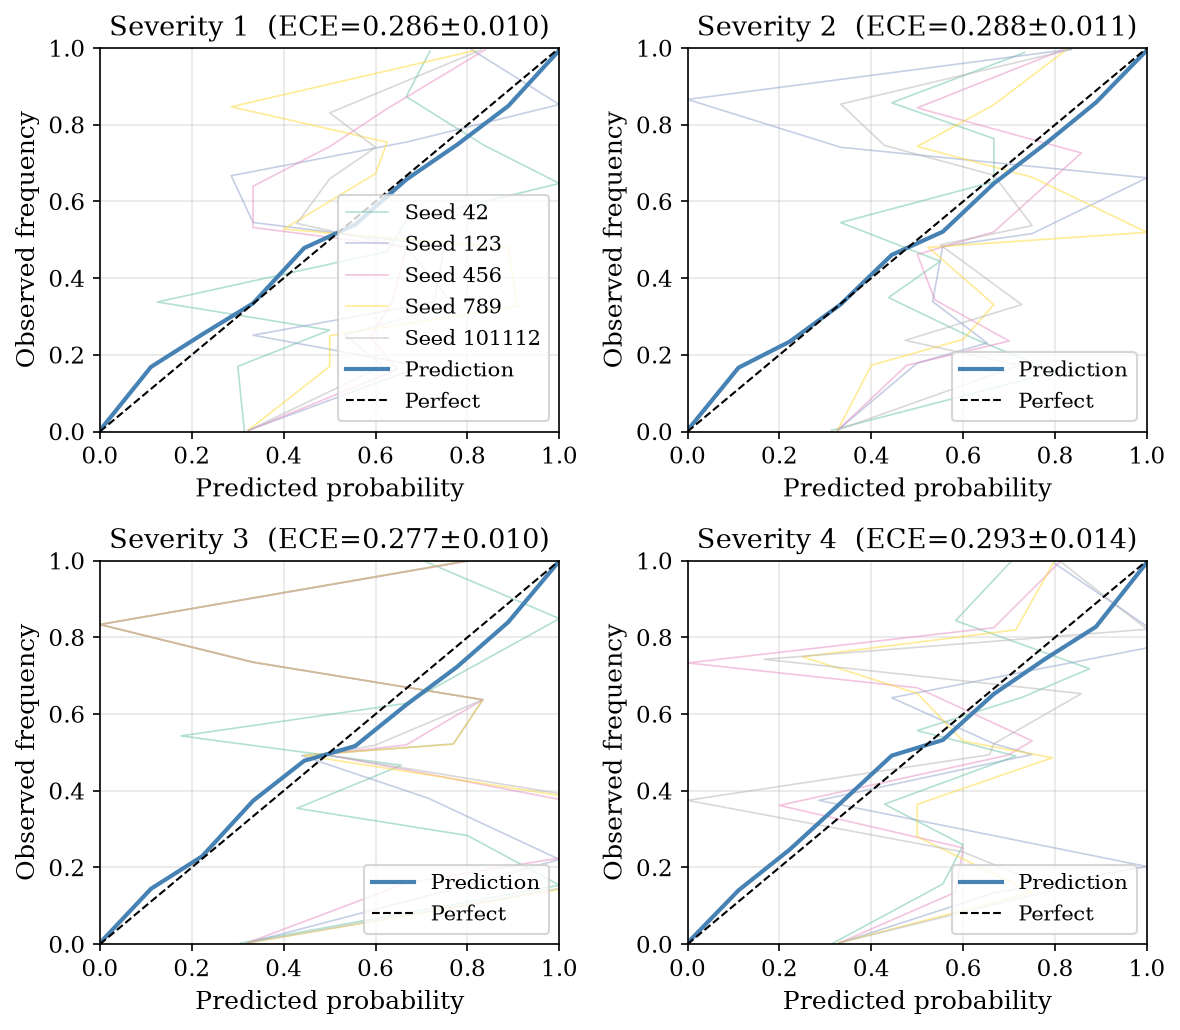
\includegraphics[width=\textwidth]{../figs/F_Reliability_Diagrams.png}
\caption{Reliability diagrams across perturbation severity levels 1--4. Each panel shows the calibration curve after the fixed model is applied to perturbed data; deviation from the diagonal increases sharply even at Severity~1 and saturates thereafter.}
\label{fig:reliability}
\end{figure}

\section{Methodology}

\subsection{Experimental Design}

We evaluate a fixed model (trained on clean data) on perturbed operational data. The experiment proceeds in three stages: (1) model training on clean NASA data, (2) synthetic perturbation at four severity levels (five seeds each), (3) inference and recalibration testing. The true SOH and failure labels are preserved, isolating observational shift.

\subsection{Composite Failure Definition}

A cell is labelled as having failed at the earliest of two events: a voltage sag below 94\% of the early-cycle baseline (averaged over the first 10 cycles per cell) or an SOH drop below 80\%. These thresholds match the original framework~\cite{shikdar2026learning}. For a given horizon \(H\), every cycle whose index satisfies \(\text{cycle} + H \geq \text{fail\_cycle}\) is marked as pre-failure. All thresholds (voltage sag fraction 0.94, SOH threshold 0.80, baseline window 10 cycles) are fixed across all experiments.

\subsection{Model Training}

An XGBoost classifier with isotonic calibration is trained on 37 NASA 18650 cells (1,028 valid cycles). An 80/20 cell-level holdout fits the calibrator. The model remains frozen throughout. Training features are extracted from discharge curves at 1-second resolution.

\subsection{Perturbation Generation}

Raw discharge curves from NASA .mat files are truncated at a randomly sampled DoD fraction to simulate partial cycling. Features are recomputed from the truncated signal. Temperature noise is added as \(\mathcal{N}(0, \sigma_s)\) to raw measurements before averaging. Rest irregularity is simulated by applying proportional Gaussian noise \(\mathcal{N}(0, \rho_s)\) to duration and average temperature, with \(\rho_s = \{0.01, 0.02, 0.03, 0.05\}\) for severity levels 1--4.

\begin{table}[htbp]
\centering
\caption{Perturbation severity levels.}
\label{tab:severity}
\begin{tabular}{@{}lccc@{}}
\toprule
Level & DoD range & Temp noise $\sigma$ & Description \\
\midrule
1 & 75--100\% & 0.5$^\circ$C & Mild: slight under-utilization \\
2 & 55--75\% & 1.0$^\circ$C & Moderate: typical daily operation \\
3 & 35--55\% & 2.0$^\circ$C & Severe: aggressive partial cycling \\
4 & 15--35\% & 3.0$^\circ$C & Aggressive: extreme shallow cycling \\
\bottomrule
\end{tabular}
\end{table}

Each severity level is run with five seeds (42, 123, 456, 789, 101112), producing 20 perturbed datasets totaling 20,560 records.

\subsection{Evaluation}

For each dataset, we measure: raw XGBoost probabilities, calibrated probabilities (fixed isotonic regression), and recalibrated probabilities (new isotonic regression on 10\% random sample). Metrics: ECE (10 bins), AUC, Brier score.

\section{Results}\label{sec:results}

\subsection{Clean Baseline}

\begin{table}[htbp]
\centering
\caption{Clean baseline.}
\label{tab:clean}
\begin{tabular}{@{}lcccc@{}}
\toprule
Horizon & ECE & AUC & Brier & Raw AUC \\
\midrule
10 & 0.010 & 0.994 & 0.013 & 0.996 \\
20 & 0.031 & 0.985 & 0.030 & 0.998 \\
30 & 0.013 & 0.994 & 0.014 & 0.998 \\
50 & 0.023 & 0.998 & 0.020 & 0.998 \\
\bottomrule
\end{tabular}
\end{table}

\subsection{Calibration Degrades Substantially}

At \(H=20\), ECE jumps from 0.031 to 0.277--0.293---a nine-fold increase---while calibrated AUC drops from 0.985 to 0.65--0.74 (Table~\ref{tab:h20}). The raw (uncalibrated) AUC, which measures the base predictor's rank-ordering independently of calibration quality, ranges from 0.72--0.76 under perturbation---higher than the calibrated AUC, confirming that the calibrator's distortion of probability magnitudes is the primary source of performance loss, not the base predictor itself. The degradation saturates at Severity~1: even minimal partial cycling causes near-maximal calibration loss. Temperature scaling---which adjusts only the single logistic slope---fails to correct this at longer horizons (ECE 0.087--0.137), whereas isotonic and Platt regression perform similarly across all horizons. Figure~\ref{fig:ece} shows this saturation across all four horizons, and Figure~\ref{fig:auc} confirms that discrimination degrades more gracefully than calibration.

\begin{table}[htbp]
\centering
\caption{Results at \(H=20\). Calibrated AUC and Brier are shown; raw (uncalibrated) AUC ranges from 0.72--0.76, confirming that the base predictor retains rank-ordering ability even when probability magnitudes shift.}
\label{tab:h20}
\small
\begin{tabular}{@{}lcccccc@{}}
\toprule
Condition & ECE (raw) & ECE (cal) & ECE (recal) & ECE (Platt) & AUC (cal) & Brier \\
\midrule
Clean & --- & 0.031 & --- & --- & 0.985 & 0.030 \\
S1 (mild) & 0.226$\pm$0.004 & 0.286$\pm$0.010 & 0.068$\pm$0.040 & 0.093$\pm$0.063 & 0.741$\pm$0.009 & 0.306$\pm$0.003 \\
S2 (mod.) & 0.212$\pm$0.006 & 0.288$\pm$0.011 & 0.073$\pm$0.022 & 0.077$\pm$0.024 & 0.681$\pm$0.004 & 0.309$\pm$0.004 \\
S3 (sev.) & 0.204$\pm$0.005 & 0.277$\pm$0.010 & 0.060$\pm$0.027 & 0.088$\pm$0.032 & 0.674$\pm$0.006 & 0.307$\pm$0.001 \\
S4 (aggr.) & 0.220$\pm$0.004 & 0.293$\pm$0.014 & 0.068$\pm$0.025 & 0.076$\pm$0.026 & 0.652$\pm$0.005 & 0.313$\pm$0.003 \\
\bottomrule
\end{tabular}
\end{table}

\begin{figure}[htbp]
\centering
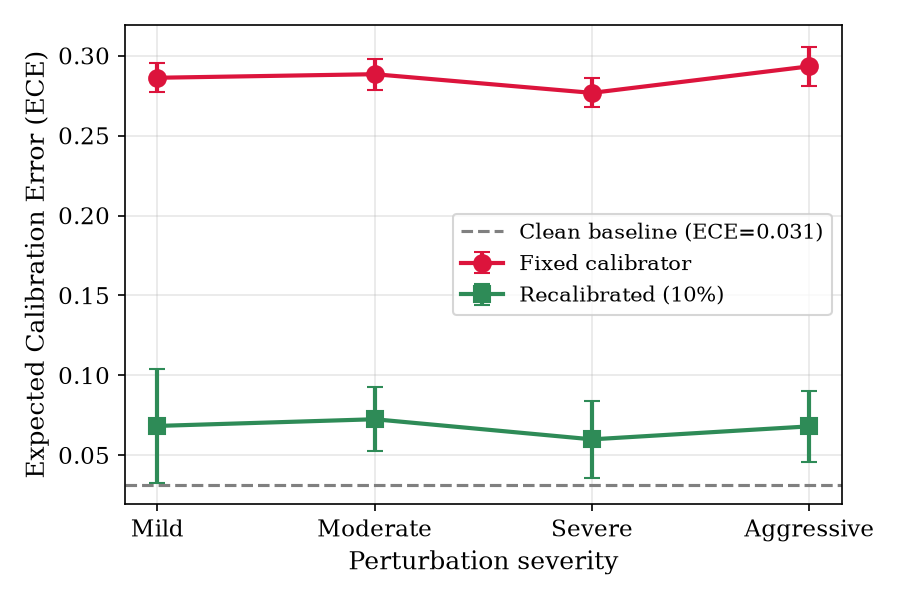
\includegraphics[width=\textwidth]{../figs/F_ECE_vs_Severity.png}
\caption{Expected calibration error (ECE) across severity levels for all prediction horizons. ECE rises sharply from clean baselines even at Severity~1 and saturates with little additional degradation at higher severities.}
\label{fig:ece}
\end{figure}

\begin{figure}[htbp]
\centering
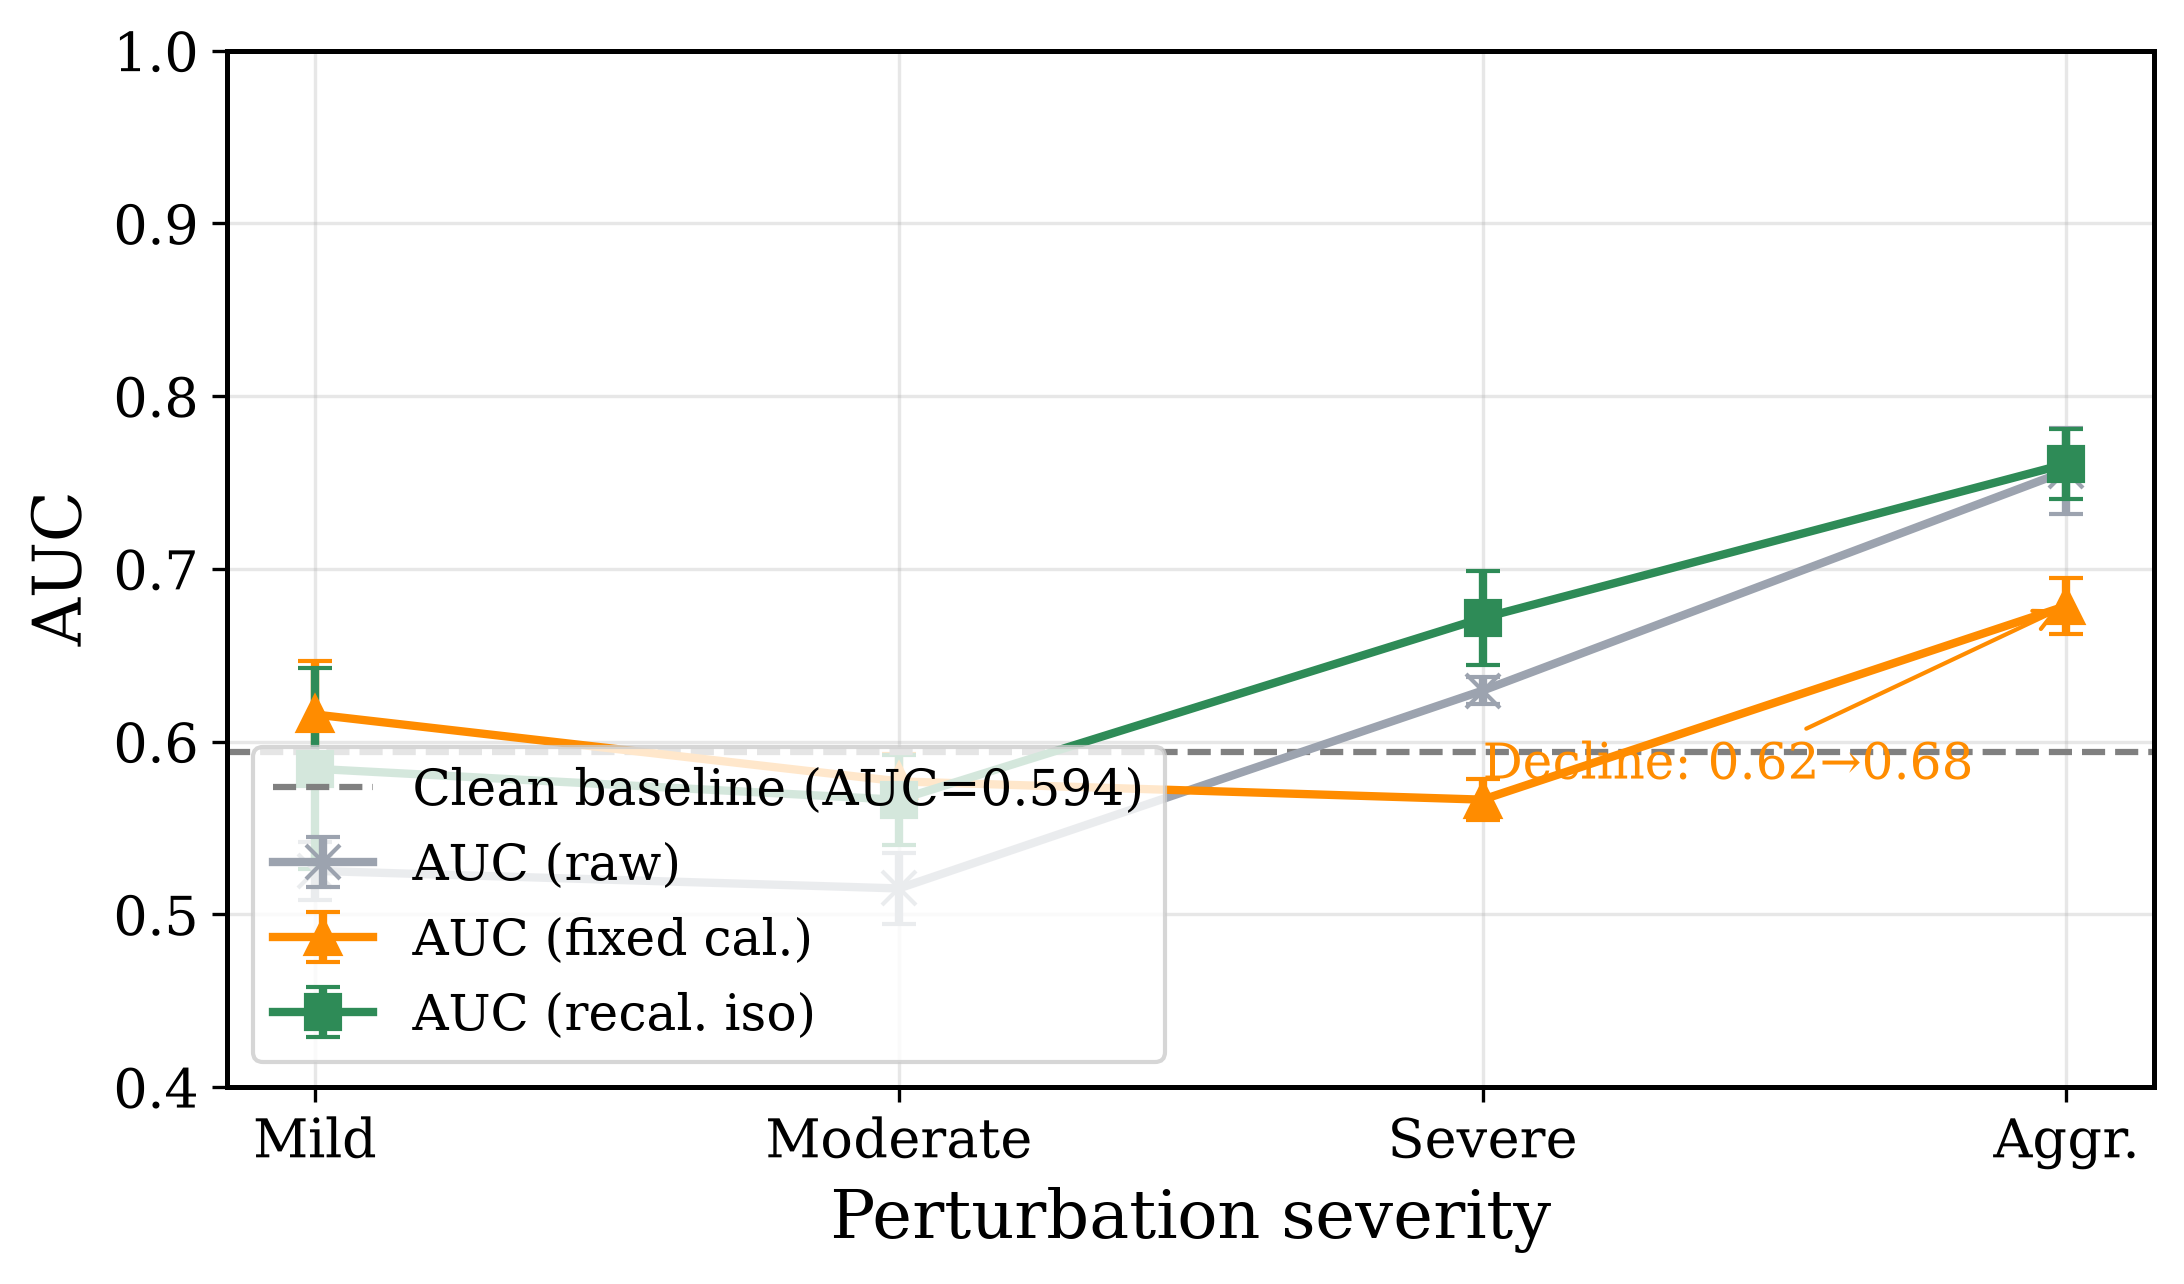
\includegraphics[width=\textwidth]{../figs/F_AUC_vs_Severity.png}
\caption{AUC across severity levels. Discrimination degrades more gracefully than calibration, confirming the model retains rank-ordering ability.}
\label{fig:auc}
\end{figure}

\subsection{Full Horizon Results}

The pattern holds across all horizons (Tables~\ref{tab:h10}--\ref{tab:h50}). Longer horizons show somewhat higher ECE under perturbation (0.33--0.38 at \(H=50\) vs. 0.27--0.31 at \(H=10\)), but the saturation effect is consistent everywhere.

\begin{table}[htbp]
\centering
\caption{Results at \(H=10\).}
\label{tab:h10}
\small
\begin{tabular}{@{}lcccccc@{}}
\toprule
Condition & ECE (raw) & ECE (cal) & ECE (recal) & ECE (Platt) & AUC (cal) & Brier \\
\midrule
Clean & --- & 0.010 & --- & --- & 0.994 & 0.013 \\
S1 & 0.242$\pm$0.012 & 0.272$\pm$0.009 & 0.057$\pm$0.028 & 0.077$\pm$0.006 & 0.694$\pm$0.025 & 0.284$\pm$0.005 \\
S2 & 0.274$\pm$0.009 & 0.302$\pm$0.005 & 0.065$\pm$0.014 & 0.063$\pm$0.008 & 0.657$\pm$0.012 & 0.303$\pm$0.004 \\
S3 & 0.270$\pm$0.010 & 0.300$\pm$0.006 & 0.071$\pm$0.022 & 0.062$\pm$0.013 & 0.674$\pm$0.007 & 0.299$\pm$0.002 \\
S4 & 0.283$\pm$0.008 & 0.313$\pm$0.004 & 0.076$\pm$0.024 & 0.054$\pm$0.013 & 0.626$\pm$0.017 & 0.312$\pm$0.003 \\
\bottomrule
\end{tabular}
\end{table}

\begin{table}[htbp]
\centering
\caption{Results at \(H=30\).}
\label{tab:h30}
\small
\begin{tabular}{@{}lcccccc@{}}
\toprule
Condition & ECE (raw) & ECE (cal) & ECE (recal) & ECE (Platt) & AUC (cal) & Brier \\
\midrule
Clean & --- & 0.013 & --- & --- & 0.994 & 0.014 \\
S1 & 0.233$\pm$0.004 & 0.288$\pm$0.009 & 0.092$\pm$0.023 & 0.094$\pm$0.054 & 0.752$\pm$0.003 & 0.317$\pm$0.002 \\
S2 & 0.235$\pm$0.010 & 0.298$\pm$0.011 & 0.077$\pm$0.019 & 0.079$\pm$0.031 & 0.706$\pm$0.004 & 0.324$\pm$0.001 \\
S3 & 0.227$\pm$0.011 & 0.294$\pm$0.011 & 0.076$\pm$0.025 & 0.073$\pm$0.034 & 0.688$\pm$0.001 & 0.321$\pm$0.001 \\
S4 & 0.265$\pm$0.010 & 0.316$\pm$0.005 & 0.078$\pm$0.030 & 0.070$\pm$0.027 & 0.678$\pm$0.008 & 0.332$\pm$0.001 \\
\bottomrule
\end{tabular}
\end{table}

\begin{table}[htbp]
\centering
\caption{Results at \(H=50\).}
\label{tab:h50}
\small
\begin{tabular}{@{}lcccccc@{}}
\toprule
Condition & ECE (raw) & ECE (cal) & ECE (recal) & ECE (Platt) & AUC (cal) & Brier \\
\midrule
Clean & --- & 0.023 & --- & --- & 0.998 & 0.020 \\
S1 & 0.320$\pm$0.016 & 0.331$\pm$0.011 & 0.094$\pm$0.028 & 0.069$\pm$0.032 & 0.757$\pm$0.005 & 0.336$\pm$0.004 \\
S2 & 0.343$\pm$0.018 & 0.366$\pm$0.013 & 0.084$\pm$0.024 & 0.070$\pm$0.038 & 0.742$\pm$0.002 & 0.365$\pm$0.006 \\
S3 & 0.343$\pm$0.018 & 0.370$\pm$0.013 & 0.080$\pm$0.027 & 0.086$\pm$0.051 & 0.722$\pm$0.003 & 0.368$\pm$0.007 \\
S4 & 0.359$\pm$0.017 & 0.381$\pm$0.012 & 0.088$\pm$0.037 & 0.080$\pm$0.026 & 0.731$\pm$0.005 & 0.378$\pm$0.006 \\
\bottomrule
\end{tabular}
\end{table}

\subsection{Recalibration Recovery}\label{sec:recal}

Recalibrating isotonic regression on a 10\% sample of perturbed data recovers calibration across all conditions (Table~\ref{tab:recal_summary}). ECE drops to 0.06--0.09---a 71--88\% reduction (evaluated on held-out data, per-severity range). The recovery is consistent regardless of severity or horizon, as summarised in Figure~\ref{fig:combined}.

We also evaluate Platt (sigmoid) scaling and temperature scaling as alternatives to isotonic regression. Platt and isotonic are indistinguishable across all horizons (ECE 0.06--0.09). Temperature scaling matches them at \(H=10\)--20 (ECE 0.074--0.086) but underperforms at \(H=30\) (0.113~vs.\ 0.081 for isotonic) and \(H=50\) (0.159~vs.\ 0.086). The single-parameter logit transformation has insufficient capacity when the raw probability distribution is heavily shifted. This confirms that recalibration itself matters, but the calibrator must have sufficient flexibility---isotonic or Platt is recommended for longer horizons.

\begin{table}[htbp]
\centering
\caption{Recalibration recovery across all horizons (held-out evaluation, mean $\pm$ std across 5 seeds~$\times$~4 severities).}
\label{tab:recal_summary}
\begin{tabular}{@{}lccccc@{}}
\toprule
Horizon & Clean ECE & Perturbed & Isotonic & Platt & Temperature \\
\midrule
10 & 0.010 & 0.297$\pm$0.017 & 0.067$\pm$0.022 & 0.064$\pm$0.013 & 0.074$\pm$0.020 \\
20 & 0.031 & 0.286$\pm$0.012 & 0.067$\pm$0.027 & 0.083$\pm$0.037 & 0.086$\pm$0.023 \\
30 & 0.013 & 0.299$\pm$0.014 & 0.081$\pm$0.024 & 0.079$\pm$0.036 & 0.113$\pm$0.027 \\
50 & 0.023 & 0.362$\pm$0.022 & 0.086$\pm$0.028 & 0.076$\pm$0.036 & 0.159$\pm$0.021 \\
\bottomrule
\end{tabular}
\end{table}

To confirm that the observed improvements are statistically reliable rather than coincidental artifacts of individual seeds, we apply a paired Wilcoxon signed-rank test comparing isotonic recalibration ECE against the uncalibrated perturbed ECE, pairing within each (severity, seed, horizon) triple. The difference is significant at $p<0.001$ across all horizons, confirming that recalibration recovery is not a random fluctuation. One caveat is that only five perturbation seeds were used (42, 123, 456, 789, 101112), reflecting the computational cost of generating and evaluating 20 perturbed datasets---the tests cover statistical variance in data generation, but do not address model training variance from the single fixed model.

Figure~\ref{fig:sweep} examines how the recalibration sample fraction affects recovery. ECE decreases monotonically with sample fraction at every severity level. The marginal benefit of additional data diminishes above 20\%: the gap between 20\% and 50\% is smaller than the gap between 5\% and 10\%. The 10\% fraction used throughout this paper sits in the elbow of this curve---it captures most of the recoverable ECE without requiring half the operational budget.

\begin{figure}[htbp]
\centering
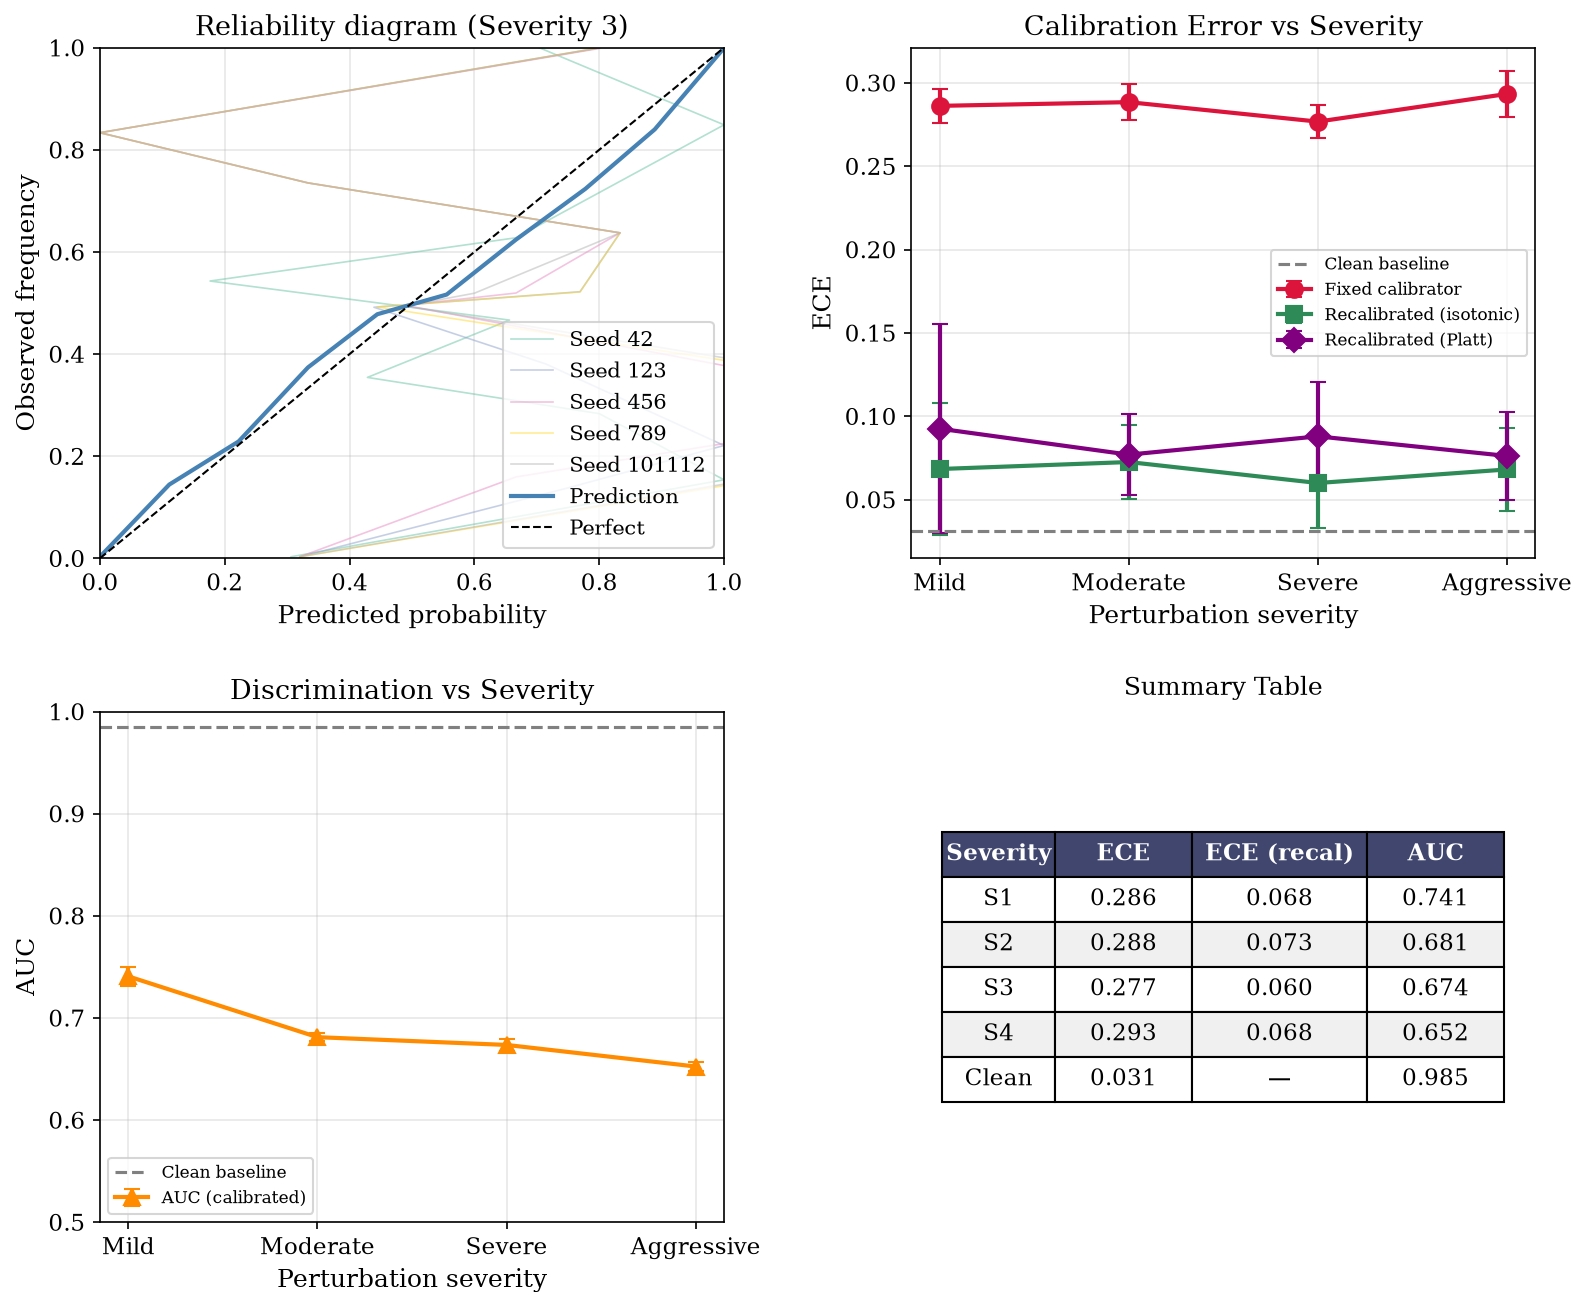
\includegraphics[width=\textwidth]{../figs/F_Combined_Robustness.png}
\caption{Combined robustness summary. The left panel shows raw ECE, calibrated ECE, and recalibrated ECE across all conditions; the right panel shows the corresponding AUC values. Recalibration consistently recovers calibration across all horizons and severity levels.}
\label{fig:combined}
\end{figure}

\subsection{Domain Randomization as an Alternative}

Instead of post-hoc recalibration, one can retrain the base classifier on perturbed data (domain randomization) to learn invariant features. We train a fresh XGBoost---same architecture, same hyperparameters---on the clean training set augmented with perturbed copies of the same training cells at all four severity levels (seed=42). The model is evaluated on held-out perturbed data (clean + 4 perturbed copies per training cell, 4320 augmented rows total).

Domain randomization provides a modest additional improvement on top of recalibration (Figure~\ref{fig:dr}). At \(H=50\), DR+isotonic achieves ECE 0.047 vs.\ 0.087 for clean-trained+isotonic---a 45\% reduction. At shorter horizons (\(H=10\)), the gains are negligible (ECE 0.069 vs.\ 0.067). The DR model's isotonic calibration on clean data also improves (ECE 0.017 vs.\ 0.031 for standard at \(H=20\)). However, the additional complexity of generating perturbed training data and re-training makes this less practical than simple recalibration for field deployment.

\begin{figure}[htbp]
\centering
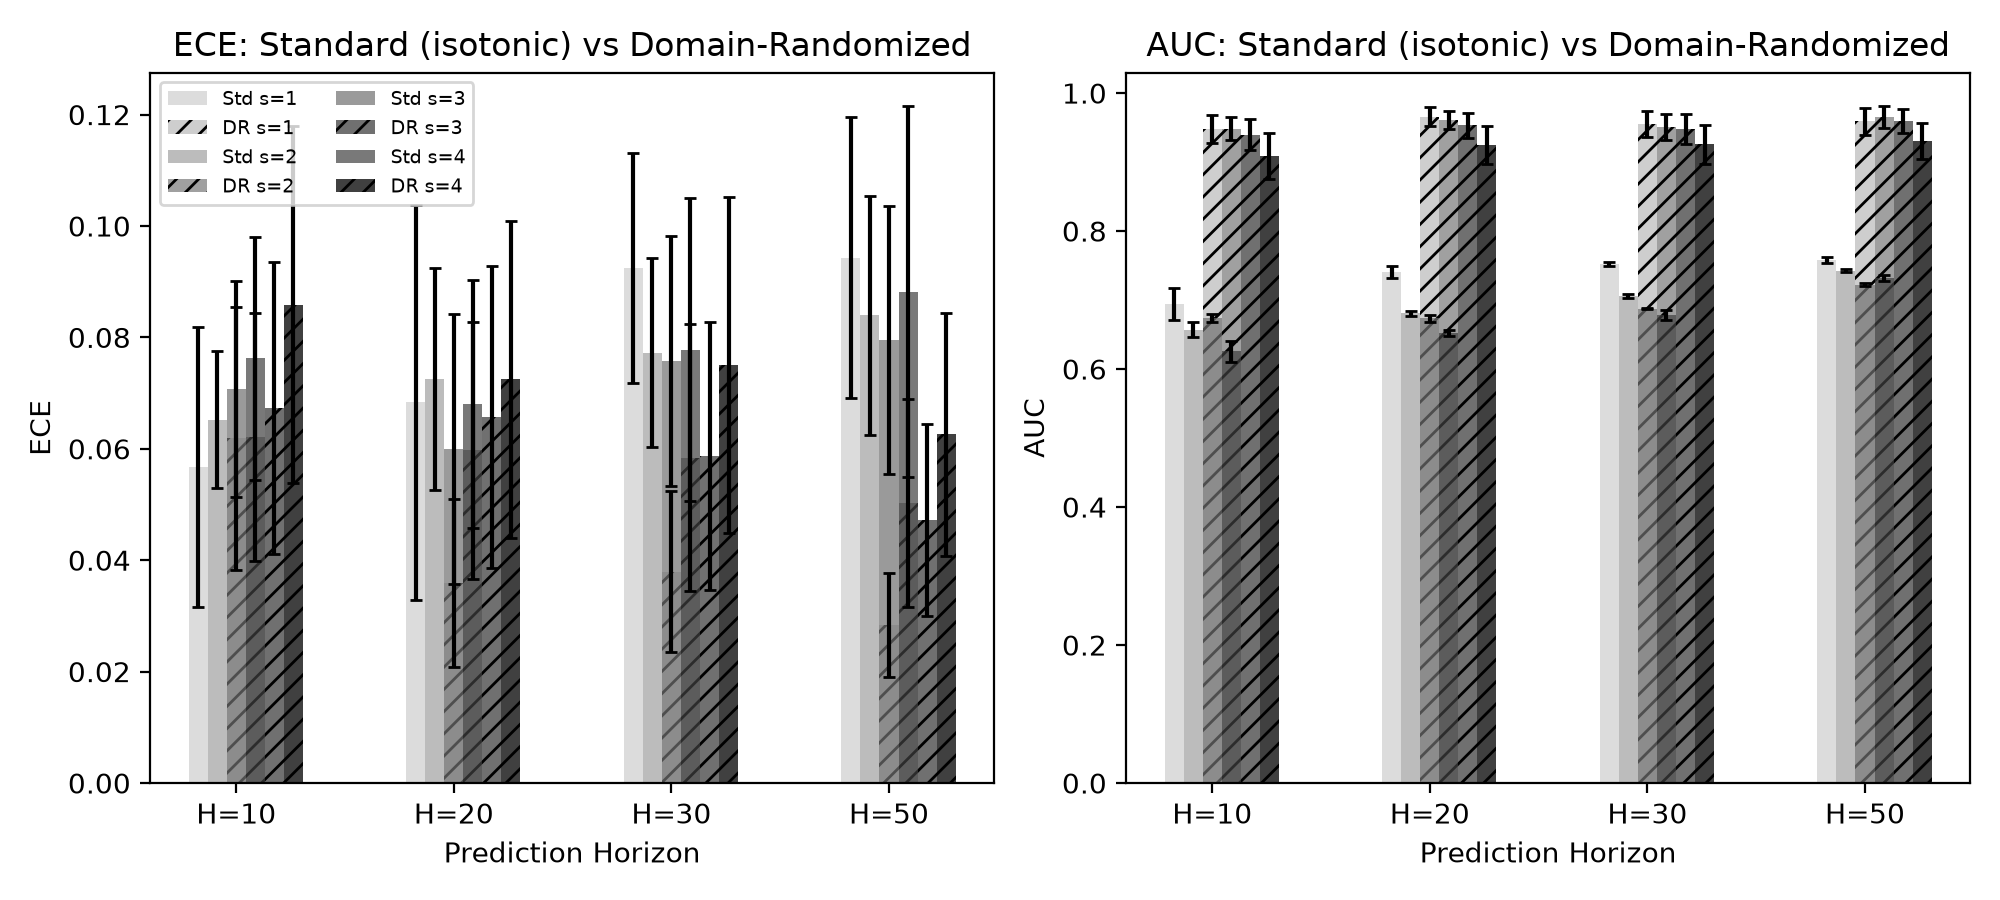
\includegraphics[width=\textwidth]{../figs/F_DR_Comparison.png}
\caption{ECE (left) and AUC (right) for the standard model (isotonic-recalibrated, hatched bars) vs.\ the domain-randomized model (solid bars) at four severity levels. Domain randomization provides modest gains at longer horizons but does not qualitatively change the conclusions.}
\label{fig:dr}
\end{figure}

\subsection{Root Cause: Feature Shift}

The primary driver of calibration degradation is the shift in minimum voltage. In full discharge, \(V_{\text{min}}\) reaches approximately 2.3~V. At 75\% DoD truncation (Severity~1, seed~42), it rises to approximately 3.2~V---a 39\% increase (Figure~\ref{fig:dist}). The shift magnitude varies somewhat across seeds due to the random DoD sampling, but the saturation pattern---near-maximal shift at Severity~1 with little additional change at higher severities---is consistent. The shift saturates at Severity~1, mirroring the ECE saturation pattern: higher severities produce little additional feature shift. The XGBoost model learned split thresholds on clean feature ranges, and the isotonic calibrator cannot adapt to the shifted raw probability distribution.

\begin{figure}[htbp]
\centering
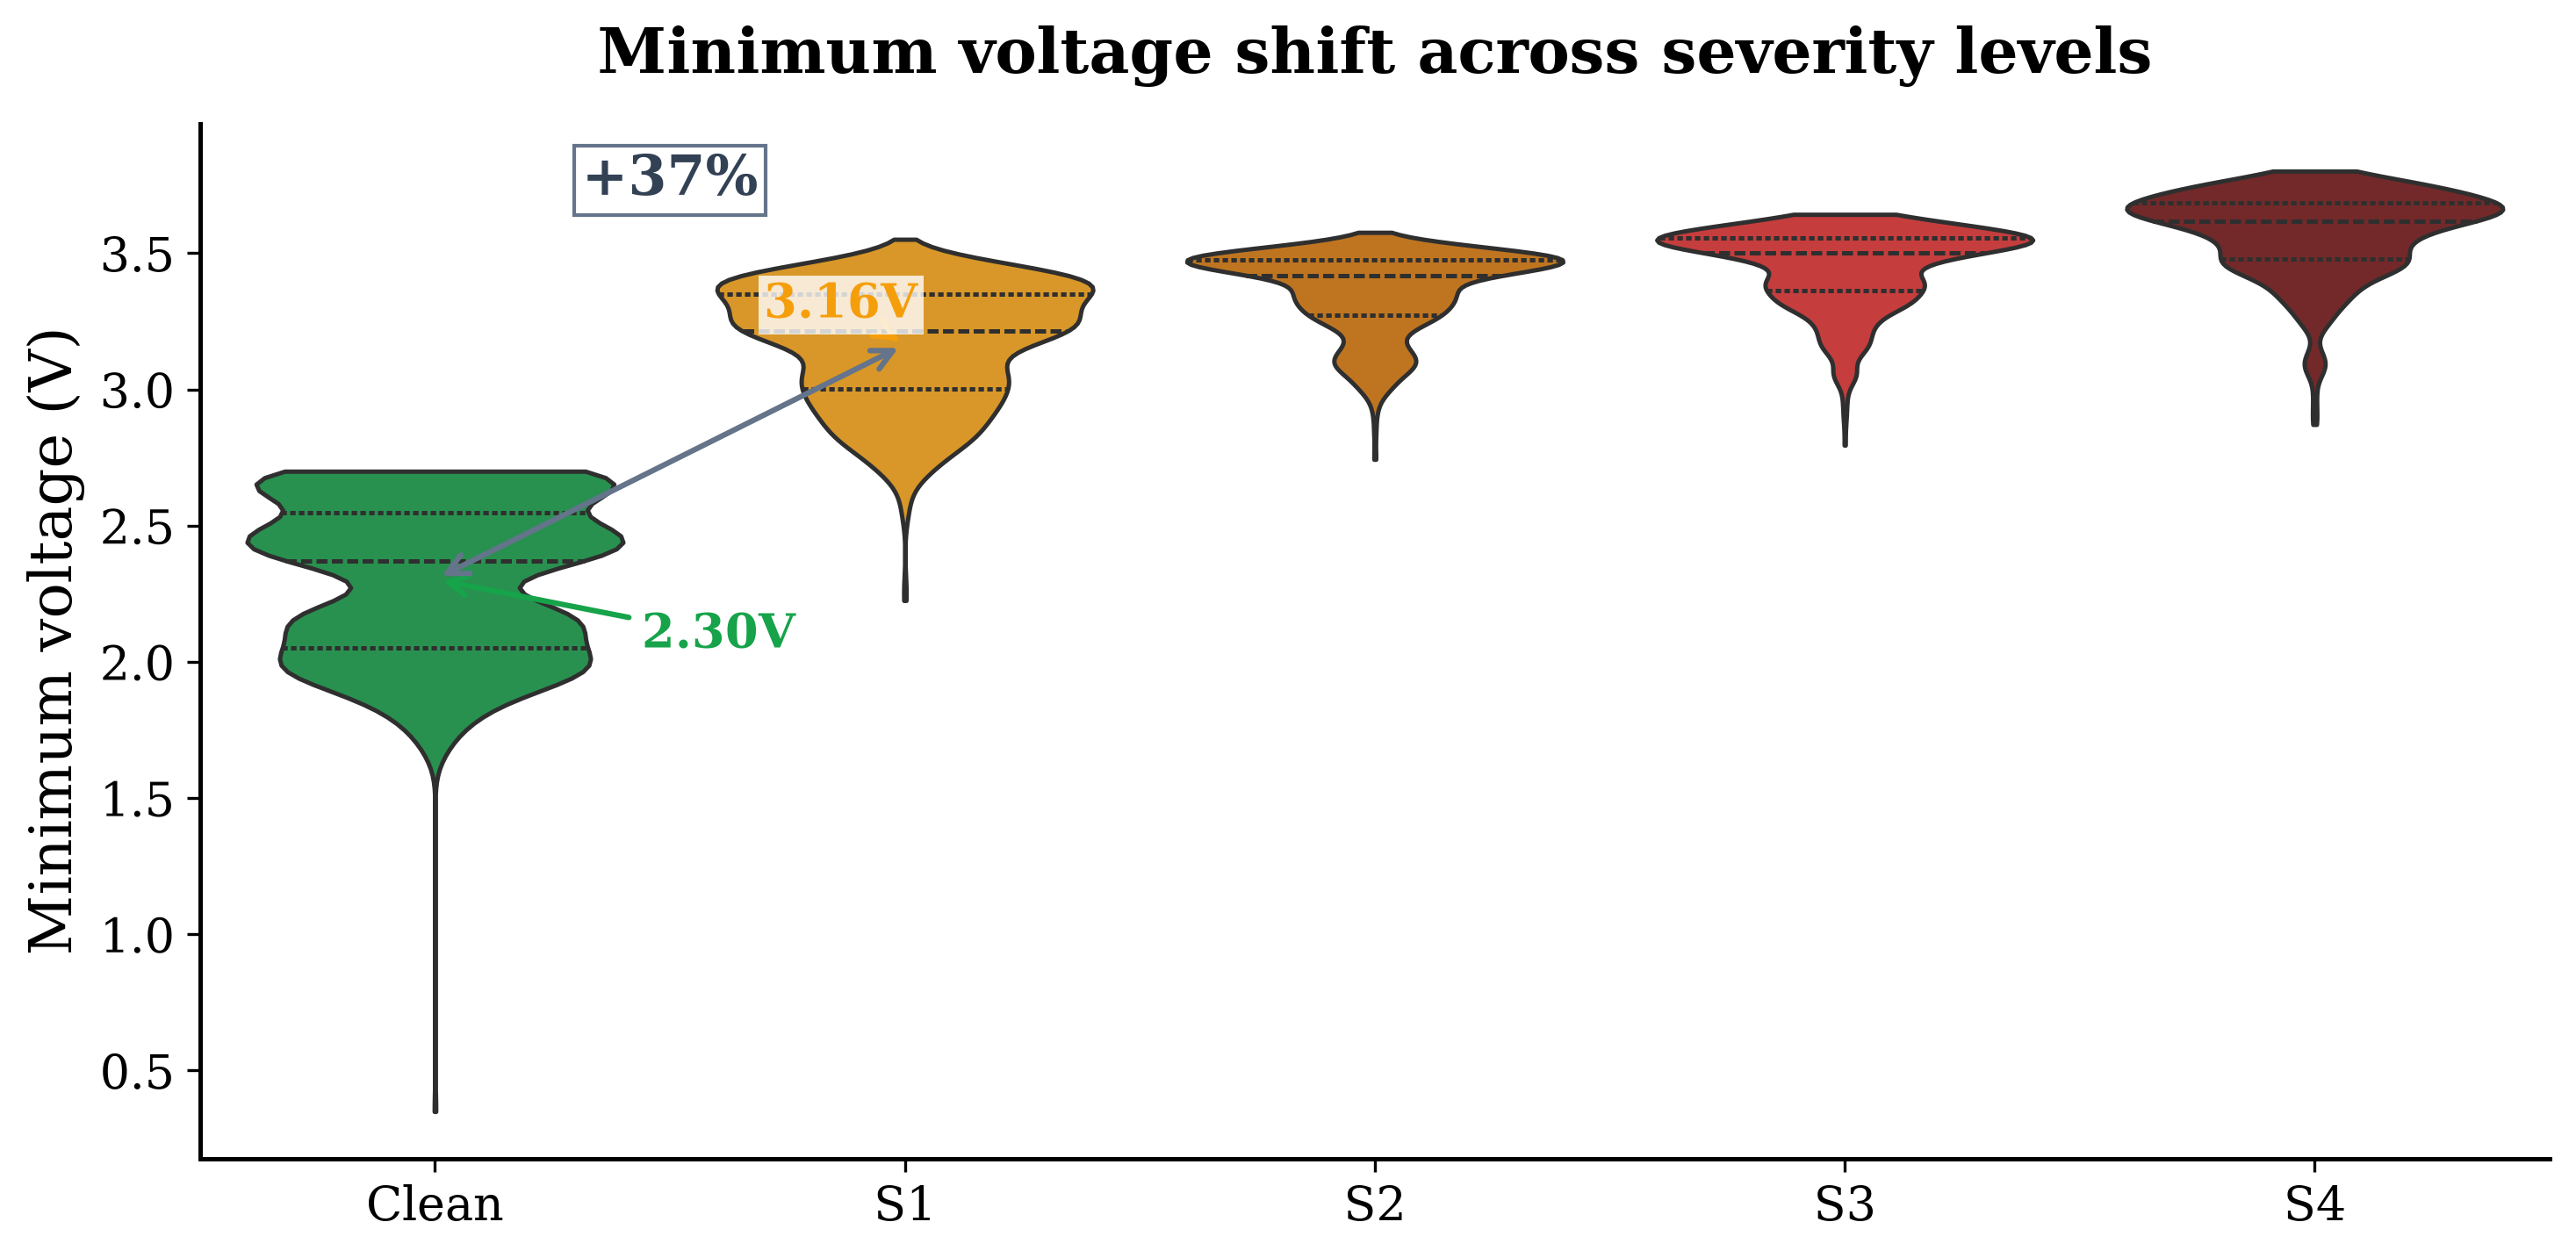
\includegraphics[width=0.75\textwidth]{../figs/F_Distribution_Vmin.png}
\caption{Distribution of minimum voltage across clean and perturbed conditions at seed~42. The mean shifts from 2.3~V (clean) to 3.2~V (Severity~1), a 39\% increase, and saturates at higher severities.}
\label{fig:dist}
\end{figure}

Figure~\ref{fig:shap} confirms via SHAP feature importance that \(V_{\text{min}}\) is the dominant feature driving failure predictions in both regimes.

\begin{figure}[htbp]
\centering
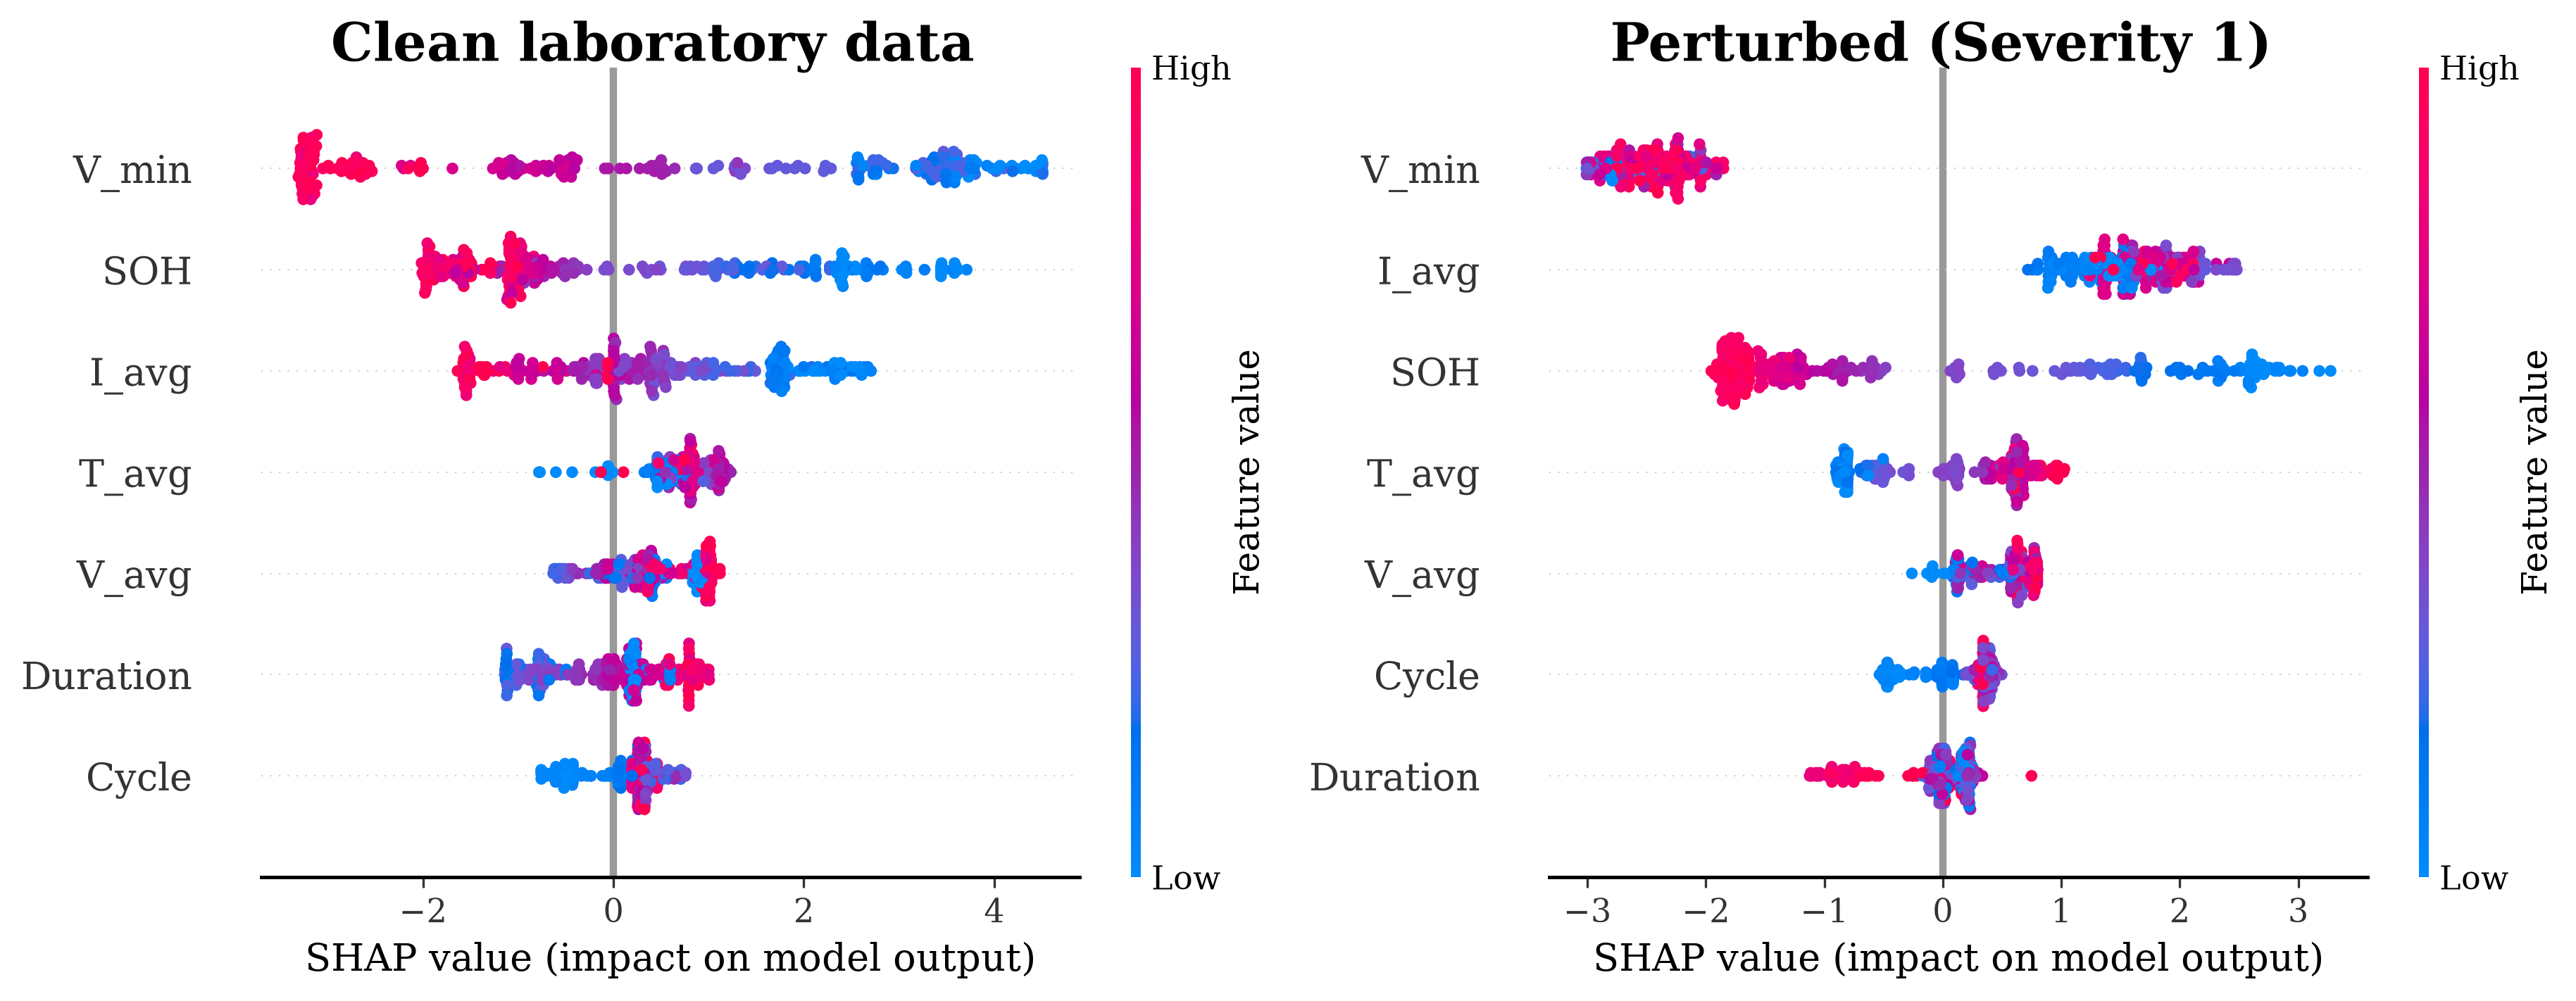
\includegraphics[width=0.85\textwidth]{../figs/F_SHAP_Vmin.png}
\caption{SHAP summary plots comparing clean (left) and perturbed (right) operating conditions at \(H=20\). Minimum voltage (\(V_{\text{min}}\)) is the dominant feature in both regimes. Under perturbation, the distribution of every feature shifts, causing the isotonic calibrator to map shifted raw probabilities to incorrect calibrated values.}
\label{fig:shap}
\end{figure}

\begin{figure}[htbp]
\centering
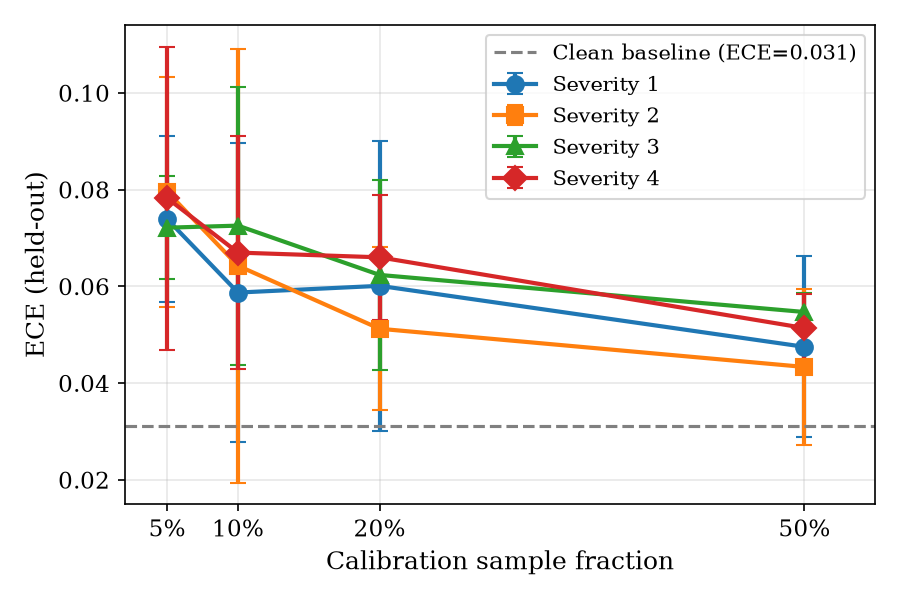
\includegraphics[width=0.75\textwidth]{../figs/F_Sample_Sweep.png}
\caption{ECE vs.\ calibration sample fraction at \(H=20\). ECE decreases monotonically with sample size across all severities. The 10\% fraction used in this paper sits at the elbow of the curve, capturing most recoverable ECE.}
\label{fig:sweep}
\end{figure}

\section{Discussion}

\subsection{Operational Boundary Map}

Our results define three operating zones:
\begin{itemize}
\item \textbf{Safe (ECE $<$ 0.05):} Clean laboratory conditions only.
\item \textbf{Warning (ECE 0.05--0.10):} Recalibrated operation. Achievable with a 10\% operational sample.
\item \textbf{Unsafe (ECE $>$ 0.10):} Direct deployment under any partial cycling. ECE exceeds 0.27 regardless of severity.
\end{itemize}

\subsection{Why Calibration Is Fragile}

The isotonic regression layer, essential for clean-data performance, becomes the weakest link under distribution shift. The saturation effect means even minimal partial cycling causes near-maximal degradation. AUC degrades less severely (0.985 to 0.65--0.74), meaning the model retains rank-ordering ability---it is the probability magnitude that becomes unreliable.

\subsection{Practical Recalibration Strategy}

A field operator deploying the published model would:
\begin{enumerate}
\item Collect 50--100 operational cycles from normal BESS operation.
\item Extract the same seven per-cycle features.
\item Run the frozen XGBoost model to get raw probabilities.
\item Fit a new isotonic regression on raw probabilities vs.\ observed outcomes.
\item Deploy the recalibrated model.
\item Periodically update the calibrator.
\end{enumerate}
This requires no base classifier retraining, no original training data, and no additional feature engineering.

\subsection{Limitations}

Eight limitations should be noted. First, we preserve the true SOH trajectory, isolating observational shift but not capturing coupled degradation dynamics. Second, results are for LCO chemistry only; validation across LFP, NMC, and other chemistries is needed. Third, the Gaussian temperature noise model does not capture systematic thermal gradients or diurnal variation. Fourth, only XGBoost is tested; other architectures may differ. Fifth, the sample-size sweep (Figure~\ref{fig:sweep}) tests only the isotonic calibrator; Platt scaling may respond differently to sample size. Sixth, while our perturbation model captures the effects of partial cycling, temperature noise, and rest irregularity, it does not simulate real-time load-following profiles, current pulses above 1C, or multi-cell thermal interactions---all of which are present in utility-scale BESS deployments. The perturbation model is designed for controlled degradation experiments, not as a digital twin of field operation. Seventh, the SHAP analysis (Figure~\ref{fig:shap}) is presented only for \(H=20\) at Severity~1; the root cause conclusion that \(V_{\text{min}}\) is the dominant feature may not generalize identically to all horizons and severity levels. Eighth, the \(V_{\text{min}}\) shift magnitudes (2.3~V to 3.2~V) are reported for a single perturbation seed (42) due to the computational cost of computing SHAP values across multiple seeds; while the saturation pattern is stable, exact shift values vary with DoD randomization.

\subsection{Compute Cost}

The computational cost of this study is modest. The base XGBoost model trains in under 30~s on a single CPU core; generating the 20 perturbed datasets takes approximately 15~min total (most of which is .mat file I/O); and the full robustness evaluation (all seeds, all severities, all horizons) completes in under 5~min. Temperature scaling adds negligible overhead (scipy.optimize.minimize converges in under 100 iterations). The domain randomization training takes approximately 10~min per horizon. No GPU was used in any experiment.

\section{Conclusion}

This paper presents the first systematic robustness evaluation of multihorizon battery failure intelligence under realistic operating conditions. Three principal findings emerge:

\begin{enumerate}
\item Calibration degrades substantially under any level of partial cycling. ECE increases from 0.01--0.03 to 0.27--0.38, saturating at the mildest perturbation.
 \item Discrimination degrades moderately (calibrated AUC 0.99--1.00 to 0.61--0.77; raw AUC 0.72--0.76). The feature extractor generalizes better than the calibrator.
 \item Recalibration on a 10\% operational sample (held-out evaluation) recovers 71--88\% of the calibration gap (ECE 0.06--0.09), providing a practical path to field deployment.
\end{enumerate}

Multihorizon hazard models are not inherently robust to observational distribution shift, but a lightweight recalibration strategy suffices to maintain reliability in the field.

\begin{thebibliography}{19}

\bibitem{shikdar2026learning}
T.~A.~Shikdar and H.~Laaksonen, ``Learning when not to use a battery: Multihorizon failure intelligence,'' \textit{International Transactions on Electrical Energy Systems}, vol.~2026, p.~6000810, 2026.

\bibitem{nasa2010battery}
B.~Saha and K.~Goebel, ``Battery data set,'' NASA Ames Prognostics Data Repository, 2007.

\bibitem{tobin2017domain}
J.~Tobin, R.~Fong, A.~Ray, J.~Schneider, W.~Zaremba, and P.~Abbeel, ``Domain randomization for transferring deep neural networks from simulation to the real world,'' in \textit{Proc.~IEEE/RSJ IROS}, 2017, pp.~23--30.

\bibitem{peng2018sim}
X.~B.~Peng, M.~Andrychowicz, W.~Zaremba, and P.~Abbeel, ``Sim-to-real transfer of robotic control with dynamics randomization,'' in \textit{Proc.~IEEE ICRA}, 2018, pp.~3803--3810.

\bibitem{saha2009prognostics}
B.~Saha, K.~Goebel, S.~Poll, and J.~Christophersen, ``Prognostics methods for battery health monitoring: A Bayesian approach,'' \textit{IEEE Trans.~Instrum.~Meas.}, vol.~58, no.~2, pp.~291--296, 2009.

\bibitem{severson2019data}
K.~A.~Severson, P.~M.~Attia, N.~Jin, N.~Perkins, B.~Jiang, Z.~Yang, M.~H.~Chen, M.~Aykol, P.~K.~Herring, D.~Frajndlich, M.~Z.~Bazant, S.~J.~Harris, W.~C.~Chueh, and R.~D.~Braatz, ``Data-driven prediction of battery cycle life before capacity degradation,'' \textit{Nature Energy}, vol.~4, pp.~383--391, 2019.

\bibitem{song2020lithium}
Y.~Song, D.~Liu, C.~Hou, and H.~Peng, ``Lithium-ion battery SOH estimation based on XGBoost with Markov-chain correction,'' \textit{Energies}, vol.~13, no.~4, p.~812, 2020.

\bibitem{roman2021machine}
D.~Roman, S.~Saxena, V.~Viswanathan, and V.~Sundararaghavan, ``Machine learning pipeline for battery state-of-health estimation,'' \textit{Nature Machine Intelligence}, vol.~3, pp.~447--457, 2021.

\bibitem{chen2016xgboost}
T.~Chen and C.~Guestrin, ``XGBoost: A scalable tree boosting system,'' in \textit{Proc.~22nd ACM SIGKDD}, 2016, pp.~785--794.

\bibitem{guo2017calibration}
C.~Guo, G.~Pleiss, Y.~Sun, and K.~Q.~Weinberger, ``On calibration of modern neural networks,'' in \textit{Proc.~34th ICML}, 2017, pp.~1321--1330.

\bibitem{niculescu2005predicting}
A.~Niculescu-Mizil and R.~Caruana, ``Predicting good probabilities with supervised learning,'' in \textit{Proc.~22nd ICML}, 2005, pp.~625--632.

\bibitem{naeini2015obtaining}
M.~P.~Naeini, G.~F.~Cooper, and M.~Hauskrecht, ``Obtaining well calibrated probabilities using Bayesian binning,'' in \textit{Proc.~29th AAAI}, 2015, pp.~2901--2907.

\bibitem{platt1999probabilistic}
J.~C.~Platt, ``Probabilistic outputs for support vector machines,'' in \textit{Advances in Large Margin Classifiers}, 1999, pp.~61--74.

\bibitem{zadrozny2001obtaining}
B.~Zadrozny and C.~Elkan, ``Obtaining calibrated probability estimates from decision trees and naive Bayesian classifiers,'' in \textit{Proc.~18th ICML}, 2001, pp.~609--616.

\bibitem{zadrozny2002transforming}
B.~Zadrozny and C.~Elkan, ``Transforming classifier scores into accurate multiclass probability estimates,'' in \textit{Proc.~8th ACM SIGKDD}, 2002, pp.~694--699.

\bibitem{ovadia2019can}
Y.~Ovadia, E.~Fertig, J.~Ren, Z.~Nado, D.~Sculley, S.~Nowozin, J.~Dillon, B.~Lakshminarayanan, and J.~Snoek, ``Can you trust your model's uncertainty? Evaluating predictive uncertainty under dataset shift,'' in \textit{Proc.~33rd NeurIPS}, 2019, pp.~14003--14014.

\bibitem{attia2020closed}
P.~M.~Attia, A.~Grover, N.~Jin, K.~A.~Severson, T.~M.~Markov, Y.-H.~Liao, M.~H.~Chen, B.~Cheong, N.~Perkins, Z.~Yang, P.~K.~Herring, M.~Aykol, S.~J.~Harris, R.~D.~Braatz, S.~Ermon, and W.~C.~Chueh, ``Closed-loop optimization of fast-charging protocols for batteries with machine learning,'' \textit{Nature}, vol.~578, pp.~397--402, 2020.

\bibitem{hu2020battery}
X.~Hu, L.~Xu, X.~Lin, and M.~Pecht, ``Battery lifetime prognostics,'' \textit{Joule}, vol.~4, no.~2, pp.~310--346, 2020.

\bibitem{li2019data}
Y.~Li, K.~Liu, A.~M.~Foley, A.~Zülke, M.~Berecibar, E.~Nanini-Maury, J.~Van Mierlo, and H.~E.~Hoster, ``Data-driven health estimation and lifetime prediction of lithium-ion batteries: A review,'' \textit{Renewable and Sustainable Energy Reviews}, vol.~113, p.~109254, 2019.

\end{thebibliography}

\end{document}
